\documentclass{article}%
\usepackage[T1]{fontenc}%
\usepackage[utf8]{inputenc}%
\usepackage{lmodern}%
\usepackage{textcomp}%
\usepackage{lastpage}%
\usepackage[head=40pt,margin=0.5in,bottom=0.6in]{geometry}%
\usepackage{graphicx}%
%
\title{\textbf{Guaidó exhorta a Europa a intensificar las sanciones contra Maduro}}%
\author{AFP}%
\date{07/03/2019}%
%
\begin{document}%
\normalsize%
\maketitle%
\textbf{URL: }%
http://www.eluniversal.com/politica/34978/guaido{-}exhorta{-}a{-}europa{-}a{-}intensificar{-}las{-}sanciones{-}contra{-}maduro\newline%
%
\textbf{Periodico: }%
EU, %
ID: %
34978, %
Seccion: %
politica\newline%
%
\textbf{Palabras Claves: }%
NO\_TIENE\newline%
%
\textbf{Derecho: }%
2.1%
, Otros Derechos: %
\newline%
%
\textbf{\textit{El presidente del Parlamento dijo que la comunidad internacional debe impedir que el dinero de los venezolanos sea "mal utilizado para asesinar a los opositores y los pueblos autóctonos"}}%
\newline%
\newline%
%
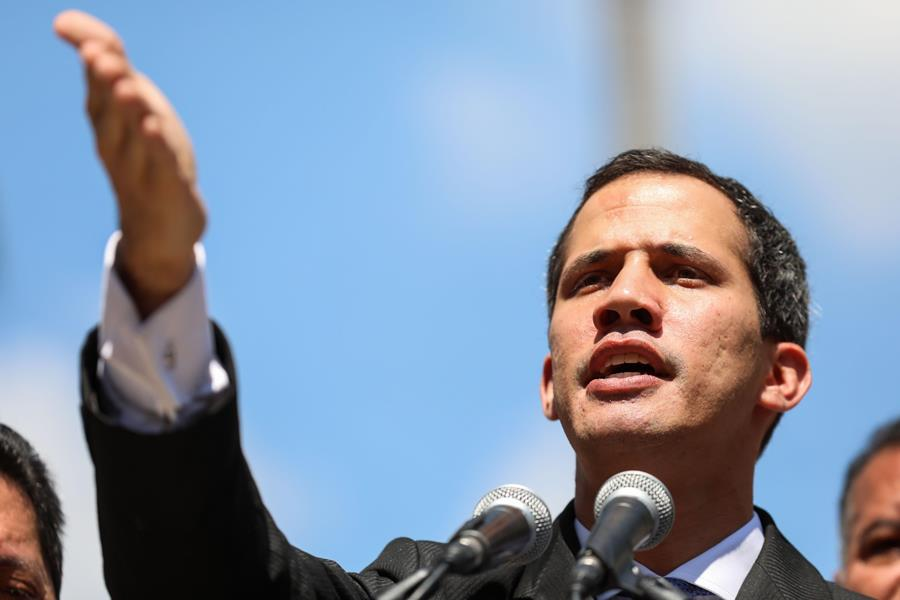
\includegraphics[width=300px]{EU_34978.jpg}%
\newline%
%
Berlín.{-}El jefe legislativo, Juan Guaidó, reconocido como presidente encargado por más de 50 países, exhortó este jueves a Europa a intensificar las sanciones financieras contra el Gobierno de Nicolás Maduro, al cual desconoce.%
\newline%
%
En declaraciones al diario alemán Spiegel, el parlamentario condenó enérgicamente la decisión del Gobierno de expulsar al embajador alemán en Venezuela, Daniel Kreiner, a quien le pidió que permanezca en el país.%
\newline%
%
Los países europeos "deben reforzar las sanciones financieras contra el régimen. La comunidad internacional debe impedir que el dinero de los venezolanos sea mal utilizado para asesinar a los opositores y los pueblos autóctonos", declaró Guaidó al diario Spiegel.%
\newline%
%
"Venezuela vive bajo una dictadura y esa manera de proceder constituye una amenaza para Alemania. Maduro ocupa ilegalmente la presidencia", acotó.%
\newline%
%
Maduro "no tiene legitimidad para declarar indeseable a un embajador", dijo Guaidó, que agradeció a Alemania por la ayuda humanitaria. \newline%
\newline%
"El régimen no solo amenaza verbalmente al embajador, sino también a su integridad física", agregó el presidente del Parlamento.%
\newline%
%
El embajador alemán Daniel Kriener fue declarado persona non grata por el Gobierno de Maduro que lo acusa de "injerencia en los asuntos internos" de Venezuela.%
\newline%
%
Alemania condenó la expulsión que considera "incomprensible" y "agrava la situación y no contribuye a la distensión".%
\newline%
%
\end{document}